\documentclass{article}

% packages with special commands
\usepackage{amssymb, amsmath}
\usepackage{epsfig}
\usepackage{array}
\usepackage{ifthen}
\usepackage{color}
\usepackage{fancyhdr}
\usepackage{graphicx}
\usepackage{mathtools}
\usepackage{csquotes}
\usepackage[authoryear]{natbib}
\usepackage{authblk}
\usepackage{hyperref}
% \usepackage[margin=1.5in]{geometry}
\definecolor{grey}{rgb}{0.5,0.5,0.5}

\newcommand{\tr}{\text{tr}}
\newcommand{\E}{\textbf{E}}
\newcommand{\diag}{\text{diag}}
\newcommand{\argmax}{\text{argmax}}
\newcommand{\Cov}{\text{Cov}}
\newcommand{\Var}{\text{Var}}
\newcommand{\argmin}{\text{argmin}}
\newcommand{\Vol}{\text{Vol}}
\newcommand{\comm}[1]{}


\begin{document}
\title{Comment on ``Causal inference using invariant prediction''}


\author{Qingyuan Zhao\thanks{Correspondence address:
    \href{mailto:qyzhao@stanford.edu}{qyzhao@stanford.edu}}
  \footnote{Contributed equally.} }

\newcommand\CoAuthorMark{\footnotemark[\arabic{footnote}]}
\author{Charles Zheng\protect\CoAuthorMark~}

\author{Trevor Hastie}

\author{Robert Tibshirani}

\affil{Department of Statistics, Stanford University}

\date{}
\maketitle

We congratulate the authors on this thought-provoking
paper. Statistical inference of causality has been thoroughly studied
in randomized experiments or observational studies, but is seldom
considered when data from both \emph{observational}
and \emph{interventional} settings are available. Peters et
al.\ made an important contribution by tackling this problem with
their notion of invariant causal prediction (ICP).

At first look, ICP is a corollary of structural
equation models, but we think its value might be much more
substantial. \citet{dawid2000causal} noticed that causal researchers
are predominately Laplacian determinists, for who
``nothing short of a functional model relating outputs to inputs will do
as a description of nature''. Peters et al.\ provide an alternative
approach that defines causality by \emph{predictability} instead
of \emph{determinism}, two different concepts that are not logically
connected \citep{hoefer2016causal}. In light of
\citet{breiman2001statistical}'s two cultures of statistics,
determinism roughly corresponds to the data modeling culture and
predictability is the spirit of Breiman's algorithmic modeling
culture.

Bearing this difference in mind, Peters et al.\ do not take a
downright predictability approach in this paper. Rather, they consider
two types of assumptions: invariant prediction in order to define
causality and deterministic modeling assumptions such as
linearity. This hybrid perspective becomes clear when comparing the
assumptions in Equation (4) to (24), (28) or (31). As a consequence,
ICP is able to make causal discovery only when the modeling
assumptions are correct. % For example, a small departure from the linear
% model can result in no causal discovery.
The authors take this as a
robustness property, but in our view it also limits the applicability in
practice. We did not find in the paper a summary of the robustness of
ICP, so we tried to outline in Table \ref{tab:icp} the behavior of
linear ICP when some of its assumptions are not met. We would welcome
the authors' comments on this summary.

\begin{table}[h]
\centering
  \begin{tabular}{c|c|c|}
    \hline
    &\textbf{Issues} & \textbf{ICP's behavior} \\
    \hline
    a) & Intervene on $Y$ (or a missing cause) &
    $\underset{\emptyset}{\bigcap}$ \\
    \hline
    b) & Non-linear, non-additive, and/or heteroscedastic &
    $\underset{\emptyset}{\bigcap}$ \\
    \hline
    c) & Not enough interventions &
    \textcolor{red}{False causal positives} \\
    \hline
    d) & Small sample size &
    $\emptyset$ \\
    \hline
    e) & Left out a confounder & $\underset{\emptyset}{\bigcap}$ \\
    \hline
    f) & Left out an unconfounding predictor & okay  \\
    \hline
    g) & Misspecified model or noise distribution & \textcolor{red}{False positives}\\\hline
  \end{tabular}
\caption{\small Robustness properties of the ICP procedure.  Under certain types
  of model misspecification, ICP will return a ``model reject'',
  denoted by $\cap_{\emptyset}$ (i.e.\ all subsets including the empty
  set are not invariant), rather than produce false positives.
(a) when interventions are performed on $Y$, no predictor set can be invariant;
(b) when the homoscedastic linear model is misspecified, the prediction rule
will vary depending on the range of the predictors; (c) without enough interventions,
the set of causal parents is unidentifiable, and non-causal invariant sets exist;
(d) when the sample size is small, the hypothesis test for invariance has insufficient power to reject the invariance null,
hence many sets are accepted as invariant;
(e) if a confounder is left out, this is equivalent to intervening on $Y$;
(f) when an uncounfounding predictor is left out, its effect is equivalent to i.i.d. noise;
(g) under a misspecified noise model, the hypothesis test may not be sensitive to differences in the noise distribution,
leading to low power.
}
\label{tab:icp}
\end{table}

To test the empirical performance of ICP, we use the authors' software
on a protein signaling network dataset. \citet{sachs2005causal}
collected a combination of observational and $9$ interventional datasets to
infer the causal structure of $11$ proteins.
Using their own method, \citet{sachs2005causal} reportedly recovered
15 of the known directed arcs and discovered two new putative links
(not shown), and missed 3 of the interactions which were known in the
literature. In contrast, ICP only makes three causal
discoveries. Among them, only one belongs to the known arcs.
The poor performance of ICP on this dataset could be explained by the
overly-restrictive linear model.

\begin{figure}[t]
\centering
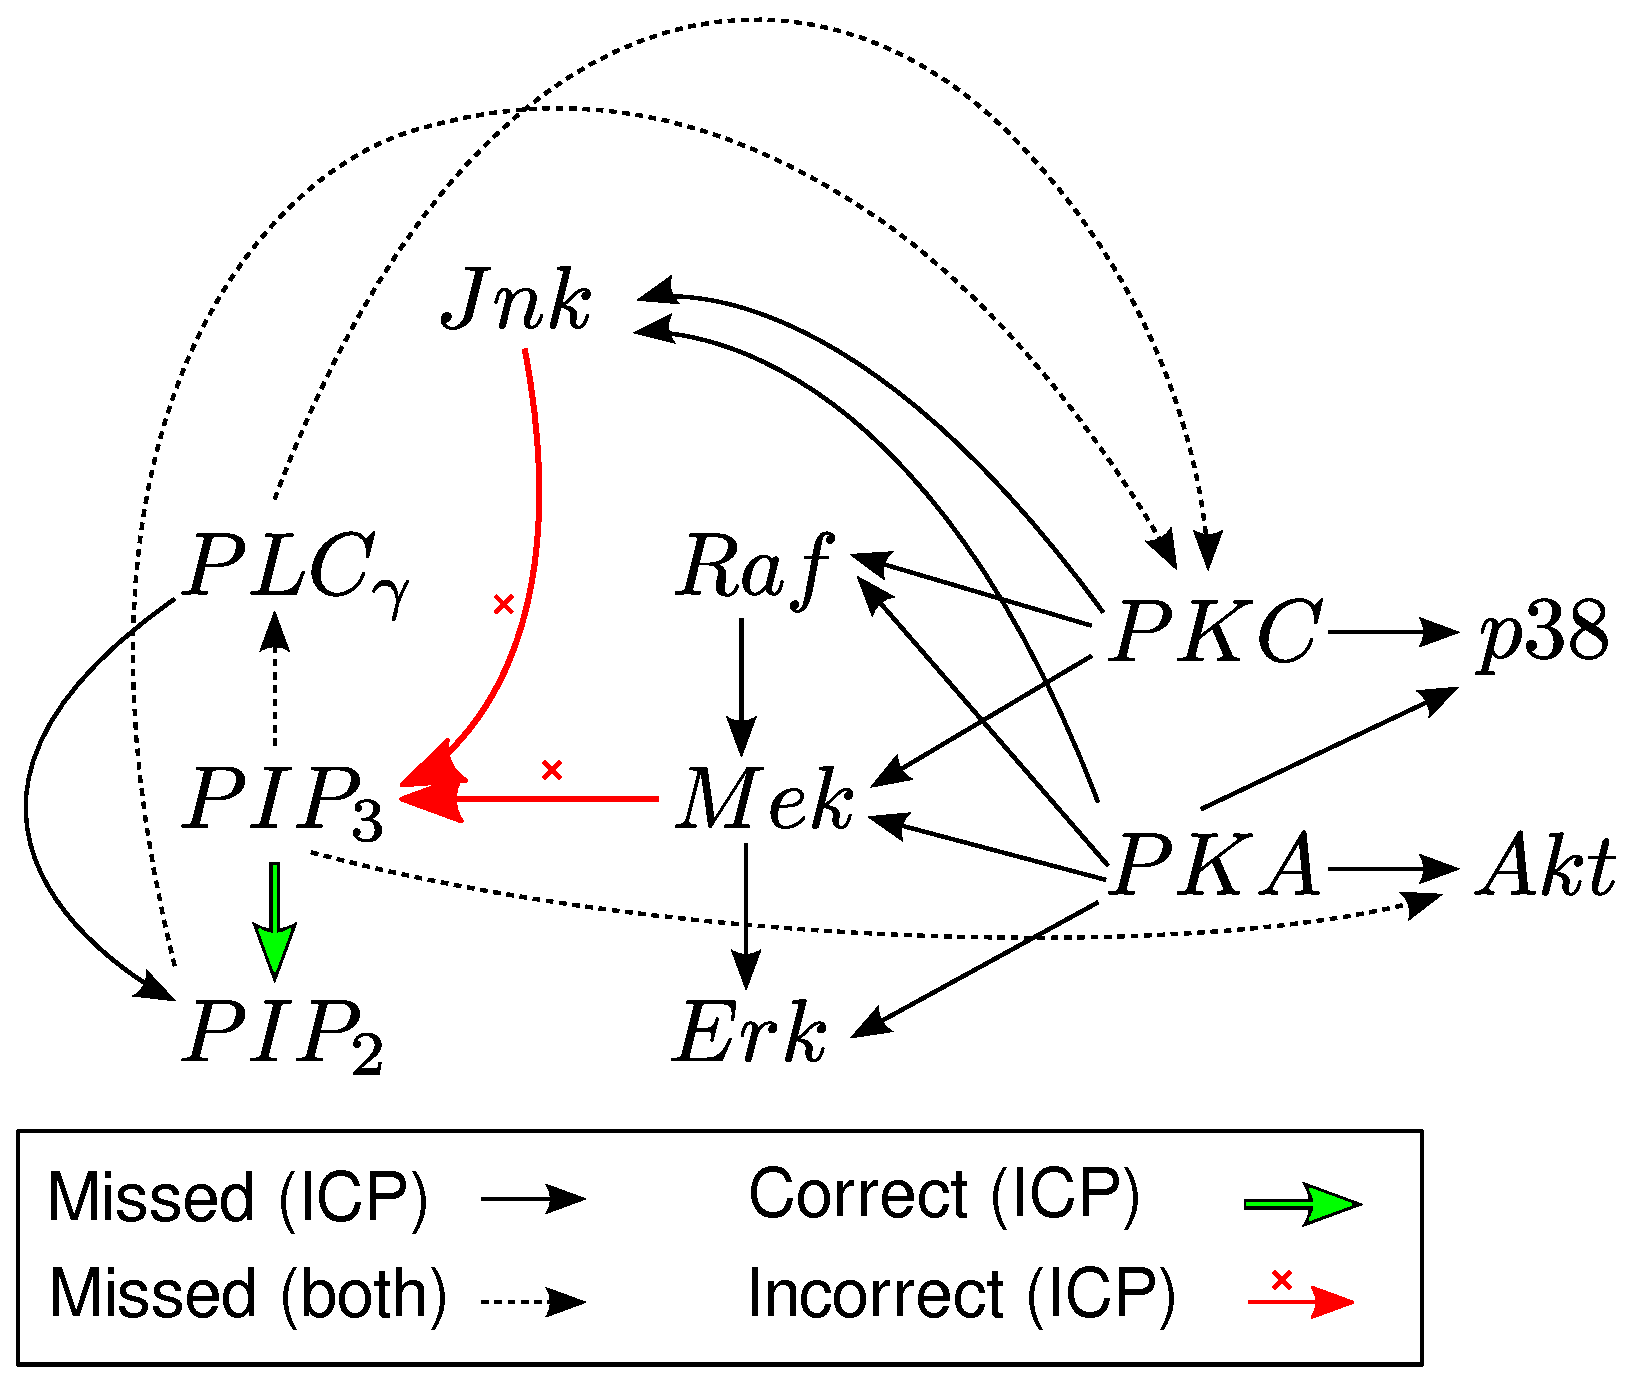
\includegraphics[scale = 0.3]{drawing2legend.eps}
\caption{\small Application of ICP procedure to recover protein signaling network,
taking in turn each of the 11 variables as the response of interest
and selecting the subset of environments in which the response was not
perturbed.  The invariant set for each variable can be identified as
the parents of that variable in the graph.  For 9 of the 11 proteins,
ICP rejected the model and reported no discoveries.  For the protein
PIP2, ICP correctly identified one parent, PIP3.  For the protein
PIP3, ICP reported Mek and Jnk as part of the invariant set, but these
do not match any interactions known in the literature.}
\label{fig:sachs}
\end{figure}

% As a final thought, ICP can be viewed as an approach to causal
% inference without counterfactuals, as advocated by
% \citet{dawid2000causal}. \citet{holland1986statistics},
% \citet{dawid2000causal} and many others suggest we should
% distinguish between the problem of ``effects of causes'' and ``causes
% of effects''. ICP answers the first question straightforwardly (when the cause of interest is not in the observed
% environments, some modularity assumptions are required).
% For the ``causes of effects'' problem, \citet{robins2000causal} and
% \citet{pearl2000comment} argue that a counterfactual language is
% necessary. Does ICP also enable us to study ``causes of effects''
% without counterfactuals? We are curious about the authors' take on
% this.

\bibliographystyle{plainnat}
\bibliography{ref}


\end{document}
